% ============================================
% SEÇÃO 3.6: ENERGIA, POTÊNCIA E DENSIDADES ESPECTRAIS
% (Unificação das antigas seções 3.7 e 3.8)
% ============================================

% ============================================
% CLASSIFICAÇÃO E DEFINIÇÕES FUNDAMENTAIS
% ============================================
\subsection{Sinais de Energia e Sinais de Potência}

\begin{frame}{Sinais de Energia e Sinais de Potência}

Todo sinal pode ser classificado pelo seu conteúdo energético:

\begin{columns}[T]
\column{0.5\textwidth}
\textbf{Energia} de um sinal:
\[
E = \int_{-\infty}^{\infty} |f(t)|^2 dt
\]

\textbf{Potência média:}
\[
P = \lim_{T \to \infty} \frac{1}{T} \int_{-T/2}^{T/2} |f(t)|^2 dt
\]

\column{0.5\textwidth}
\begin{block}{Classificação}
\begin{tabular}{lcc}
\textbf{Tipo} & $E$ & $P$ \\ \hline
Energia & finita & $0$ \\
Potência & $\infty$ & finita
\end{tabular}
\end{block}

\vspace{0.2cm}

\textbf{Nem um, nem outro:}

Sinais como $t$ ou $e^t$ têm $E = \infty$ e $P = \infty$.
\end{columns}

\vspace{0.2cm}

\textbf{Interpretação física:} Para tensão $v(t)$ em resistor de 1\,$\Omega$, $|f(t)|^2$ é a potência instantânea.

\end{frame}

% ============================================

\begin{frame}{Exemplos: Energia e Potência}

\begin{columns}[T]
\column{0.5\textwidth}
\textbf{Sinais de energia:}

Pulso retangular $A\rect(t/\tau)$:
\[
E = A^2\tau, \quad P = 0
\]

Exponencial causal $e^{-at}u(t)$:
\[
E = \frac{1}{2a}, \quad P = 0
\]

\column{0.5\textwidth}
\textbf{Sinais de potência:}

Senoide $A\cos(\omega_0 t)$:
\[
E = \infty, \quad P = \frac{A^2}{2}
\]

Constante $f(t) = A$:
\[
E = \infty, \quad P = A^2
\]

Onda quadrada $\pm A$:
\[
E = \infty, \quad P = A^2
\]
\end{columns}

\vspace{0.1cm}
{\small Ferramenta espectral: \textbf{DEE} (energia) ou \textbf{PSD} (potência).}

\end{frame}

% ============================================
% DENSIDADE ESPECTRAL DE ENERGIA (DEE)
% ============================================
\subsection{Densidade Espectral de Energia (DEE)}

\begin{frame}{Densidade Espectral de Energia}

Da Parte I, o \textbf{Teorema de Parseval} nos diz que:
\[
E = \int_{-\infty}^{\infty} |f(t)|^2\, dt = \frac{1}{2\pi} \int_{-\infty}^{\infty} |F(\omega)|^2\, d\omega
\]

Isso motiva a definição da \textbf{Densidade Espectral de Energia (DEE)}:

\begin{block}{DEE --- \textit{Energy Spectral Density (ESD)}}
\vspace{-2mm}
\[
\Psi(\omega) = |F(\omega)|^2
\]
\vspace{-2mm}
\end{block}

\begin{itemize}
\item $\Psi(\omega)$ indica quanto de energia está concentrado em cada frequência
\item Relação com energia total: $\displaystyle E = \frac{1}{2\pi} \int_{-\infty}^{\infty} \Psi(\omega)\, d\omega$
\item Para sinais reais: $\Psi(\omega)$ é par ($\Psi(-\omega) = \Psi(\omega)$)
\item Unidades: energia por rad/s (ou por Hz, se usar $f$)
\end{itemize}

\end{frame}

% ============================================

\begin{frame}{Exemplos de DEE}

\begin{columns}[T]
\column{0.5\textwidth}
\textbf{Pulso retangular} $A\rect(t/\tau)$:

$F(\omega) = A\tau \sinc\!\left(\frac{\omega\tau}{2\pi}\right)$

\[
\Psi(\omega) = A^2\tau^2 \sinc^2\!\left(\frac{\omega\tau}{2\pi}\right)
\]

\begin{itemize}
\item Máximo: $\Psi(0) = A^2\tau^2$
\item Zeros: $\omega = \pm 2\pi n/\tau$
\item Lóbulo principal: $\approx 90\%$ da energia
\end{itemize}

\column{0.5\textwidth}
\textbf{Exponencial} $e^{-at}u(t)$:

$F(\omega) = \frac{1}{a + j\omega}$

\[
\Psi(\omega) = \frac{1}{a^2 + \omega^2}
\]

\begin{itemize}
\item Lorentziana, máximo $1/a^2$
\item Banda de 3\,dB: $\omega = \pm a$
\end{itemize}

\end{columns}

\vspace{0.3cm}

\begin{center}
Verificação: $\frac{1}{2\pi}\int \Psi(\omega)\,d\omega$ coincide com $E$ calculada no tempo \checkmark
\end{center}

\end{frame}

% ============================================

\begin{frame}{Distribuição Espectral de Energia --- Simulação}

\begin{center}
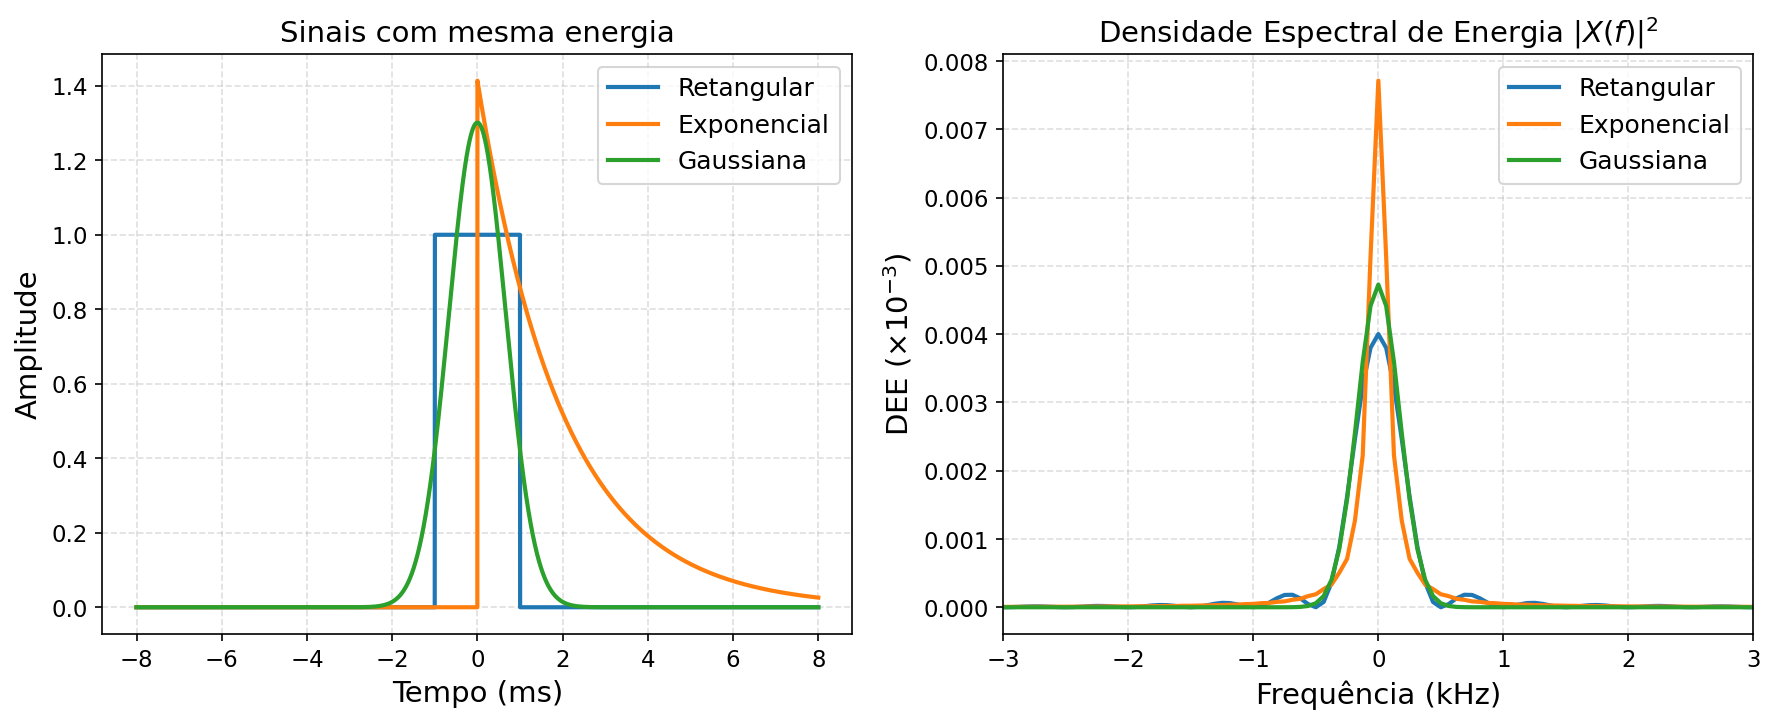
\includegraphics[width=\figFull, height=0.85\textheight, keepaspectratio]{figures/cap3/densidade_espectral_energia}
\end{center}

\end{frame}

% ============================================
% DENSIDADE ESPECTRAL DE POTÊNCIA (PSD)
% ============================================
\subsection{Densidade Espectral de Potência (PSD)}

\begin{frame}{Por que precisamos da PSD?}

Para sinais de potência, a transformada de Fourier padrão \textbf{não existe}:

\[
\int_{-\infty}^{\infty} |A\cos(\omega_0 t)|\, dt = \infty
\]

\textbf{Solução:} Truncar o sinal e normalizar pelo tempo de observação.

\begin{block}{Densidade Espectral de Potência (PSD)}
\[
S(\omega) = \lim_{T \to \infty} \frac{|F_T(\omega)|^2}{T}
\]
\end{block}

onde $f_T(t) = f(t)$ para $|t| \leq T/2$ e zero fora.

\begin{itemize}
\item Análoga à DEE, mas normalizada pelo tempo
\item Unidades: potência por Hz
\end{itemize}

\textbf{Relação com potência total:} $P = \frac{1}{2\pi} \int_{-\infty}^{\infty} S(\omega)\, d\omega$

\end{frame}

% ============================================

\begin{frame}{PSD de Sinais Periódicos}

Para sinal periódico com coeficientes de Fourier $c_n$:
\[
f(t) = \sum_{n=-\infty}^{\infty} c_n e^{jn\omega_0 t}
\]

\begin{block}{PSD de Sinal Periódico}
\[
S(\omega) = 2\pi \sum_{n=-\infty}^{\infty} |c_n|^2 \delta(\omega - n\omega_0)
\]
\end{block}

\begin{itemize}
\item Espectro discreto: impulsos nas harmônicas $\omega = n\omega_0$
\item Área de cada impulso: $2\pi|c_n|^2$ (potência naquela harmônica)
\item Potência total: $P = \sum_{n} |c_n|^2$ (Parseval para séries)
\end{itemize}

\end{frame}

% ============================================

\begin{frame}{Exemplo: PSD de Senoide}

\textbf{Sinal:} $f(t) = A\cos(\omega_0 t) = \frac{A}{2} e^{j\omega_0 t} + \frac{A}{2} e^{-j\omega_0 t}$

Coeficientes: $c_{\pm 1} = A/2$

\textbf{PSD:}
\[
S(\omega) = \frac{\pi A^2}{2} [\delta(\omega - \omega_0) + \delta(\omega + \omega_0)]
\]

\textbf{Verificação:}
\[
P = \frac{1}{2\pi} \int S(\omega)\, d\omega = \frac{1}{2\pi} \cdot \frac{\pi A^2}{2} \cdot 2 = \frac{A^2}{2} \quad \checkmark
\]

\end{frame}

% ============================================

\begin{frame}{PSD de Senoide --- Simulação}

\begin{center}
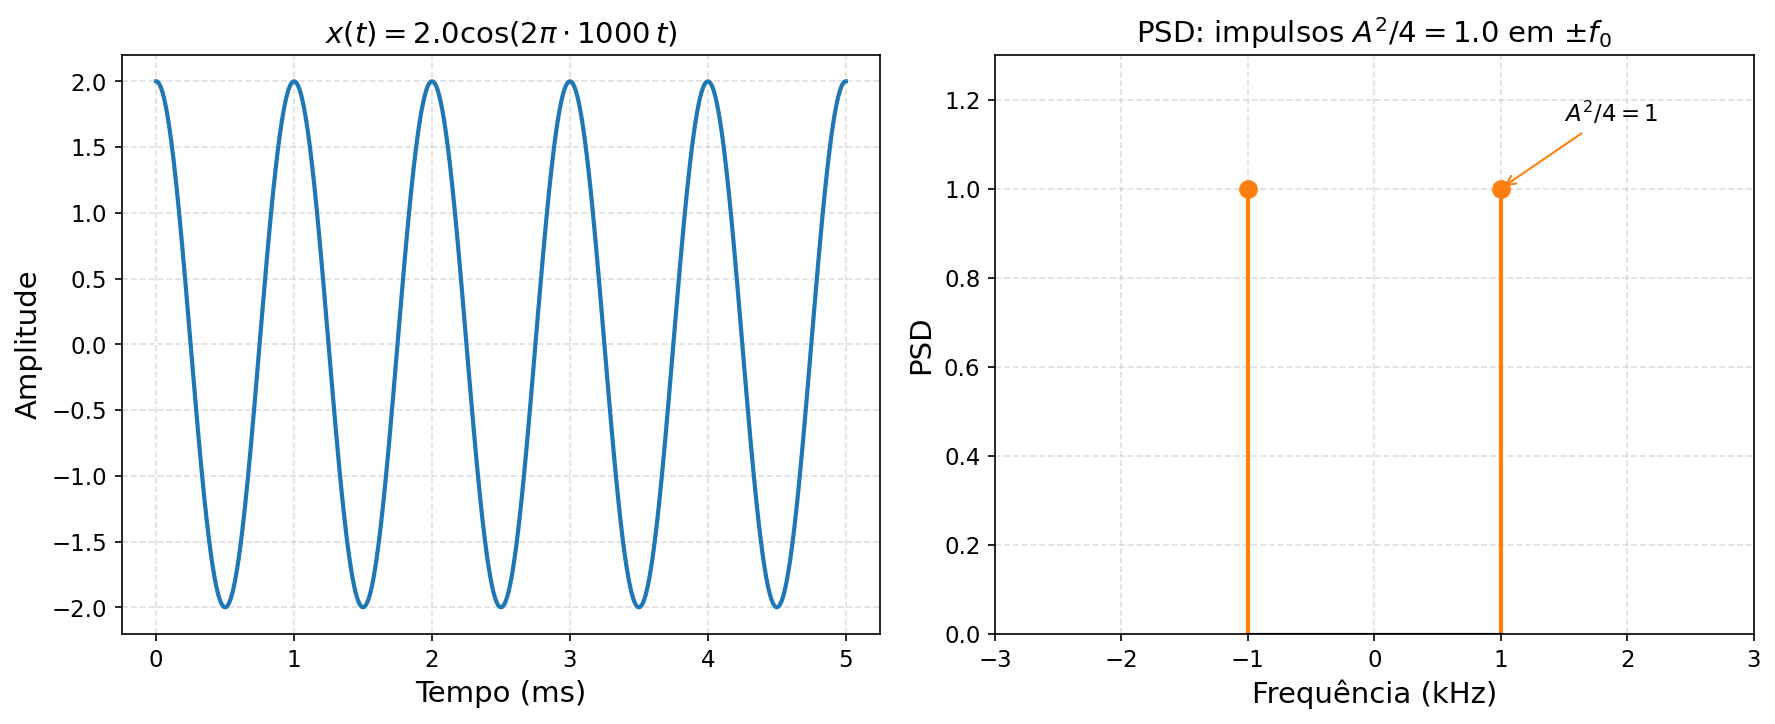
\includegraphics[width=\figFull, height=0.85\textheight, keepaspectratio]{figures/cap3/psd_senoide}
\end{center}

\end{frame}

% ============================================
% AUTOCORRELAÇÃO E WIENER-KHINCHIN (UNIFICADO)
% ============================================
\subsection{Autocorrelação e Teorema de Wiener-Khinchin}

\begin{frame}{Função de Autocorrelação}

A autocorrelação mede a \textbf{similaridade} de um sinal com versão deslocada de si mesmo.

\begin{columns}[T]
\column{0.5\textwidth}
\textbf{Sinais de energia:}
\[
R(\tau) = \int_{-\infty}^{\infty} f(t) f^*(t - \tau)\, dt
\]
\begin{itemize}
\item $R(0) = E$
\item $|R(\tau)| \leq E$
\end{itemize}

\column{0.5\textwidth}
\textbf{Sinais de potência:}
\[
R(\tau) = \lim_{T \to \infty} \frac{1}{T} \int_{-T/2}^{T/2} f(t) f^*(t - \tau)\, dt
\]
\begin{itemize}
\item $R(0) = P$
\item $|R(\tau)| \leq P$
\end{itemize}
\end{columns}

\vspace{0.3cm}

\textbf{Propriedades comuns:}

\begin{itemize}
\item $R(\tau) = R^*(-\tau)$ (simetria Hermitiana)
\item Para sinais reais: $R(\tau) = R(-\tau)$ (par)
\item Máximo em $\tau = 0$
\end{itemize}

\end{frame}

% ============================================

\begin{frame}{Teorema de Wiener-Khinchin}

A autocorrelação e a densidade espectral formam \textbf{par de Fourier}:

\begin{block}{Teorema de Wiener-Khinchin}
\[
R(\tau) \xleftrightarrow{\ft} \begin{cases} \Psi(\omega) = |F(\omega)|^2 & \text{(sinais de energia)} \\ S(\omega) & \text{(sinais de potência)} \end{cases}
\]
\end{block}

Ou seja:
\[
S(\omega) = \int_{-\infty}^{\infty} R(\tau) e^{-j\omega\tau}\, d\tau, \qquad
R(\tau) = \frac{1}{2\pi} \int_{-\infty}^{\infty} S(\omega) e^{j\omega\tau}\, d\omega
\]

\textbf{Significado:}

\begin{itemize}
\item Propriedades temporais (correlação) $\leftrightarrow$ propriedades espectrais (energia/potência)
\item PSD pode ser estimada via autocorrelação
\item Fundamental em processamento de sinais aleatórios
\end{itemize}

\end{frame}

% ============================================

\begin{frame}{Exemplo: Autocorrelação de Senoide}

\textbf{Sinal:} $f(t) = A\cos(\omega_0 t)$

Usando $\cos(a)\cos(b) = \frac{1}{2}[\cos(a-b) + \cos(a+b)]$:

\[
R(\tau) = \lim_{T \to \infty} \frac{1}{T} \int_{-T/2}^{T/2} A^2\cos(\omega_0 t)\cos(\omega_0(t-\tau))\, dt
\]

O termo $\cos(2\omega_0 t - \omega_0\tau)$ integra a zero sobre período completo:

\[
\boxed{R(\tau) = \frac{A^2}{2} \cos(\omega_0 \tau)}
\]

\textbf{Verificação via Wiener-Khinchin:}
\[
S(\omega) = \ft\{R(\tau)\} = \frac{\pi A^2}{2}[\delta(\omega - \omega_0) + \delta(\omega + \omega_0)] \quad \checkmark
\]

\end{frame}

% ============================================
% ENERGIA E POTÊNCIA NA SAÍDA DO CANAL
% ============================================
\subsection{Densidades Espectrais na Saída do Canal}

\begin{frame}{Modelo de Canal LTI}

Considere um canal de comunicação modelado como sistema LTI:

\begin{center}
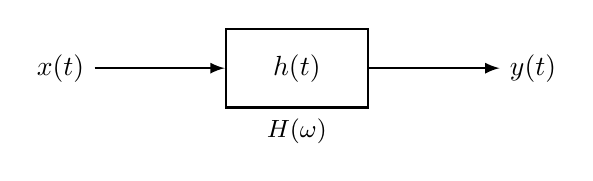
\begin{tikzpicture}[>=latex, thick]
\node (in) at (0,0) {$x(t)$};
\node[draw, minimum width=1.8cm, minimum height=1cm] (sys) at (3,0) {$h(t)$};
\node (out) at (6,0) {$y(t)$};
\draw[->] (in) -- (sys) node[midway, above] {};
\draw[->] (sys) -- (out);
\node at (3,-0.8) {\small $H(\omega)$};
\end{tikzpicture}
\end{center}

\textbf{Relações fundamentais:}

\begin{itemize}
\item No tempo: $y(t) = x(t) \conv h(t)$
\item Na frequência: $Y(\omega) = H(\omega)\, X(\omega)$
\end{itemize}

\vspace{0.2cm}

\textbf{Pergunta central:} Como a energia/potência do sinal é afetada pelo canal?

\end{frame}

% ============================================

\begin{frame}{Derivação: DEE na Saída do Canal}

\textbf{Entrada:} sinal de energia $x(t)$ com DEE $\Psi_x(\omega) = |X(\omega)|^2$.

Como $Y(\omega) = H(\omega)\, X(\omega)$, temos:

\[
|Y(\omega)|^2 = |H(\omega) X(\omega)|^2 = |H(\omega)|^2 |X(\omega)|^2
\]

\begin{block}{DEE na saída}
\[
\boxed{\Psi_y(\omega) = |H(\omega)|^2\, \Psi_x(\omega)}
\]
\end{block}

\textbf{Energia na saída} (por Parseval):

\[
E_y = \frac{1}{2\pi} \int_{-\infty}^{\infty} \Psi_y(\omega)\, d\omega = \frac{1}{2\pi} \int_{-\infty}^{\infty} |H(\omega)|^2\, |X(\omega)|^2\, d\omega
\]

O canal \textbf{redistribui} a energia: amplifica algumas frequências, atenua outras.

\end{frame}

% ============================================

\begin{frame}{Derivação: PSD na Saída do Canal}

\textbf{Entrada:} sinal de potência $x(t)$ com PSD $S_x(\omega)$.

Para o sinal truncado: $Y_T(\omega) = H(\omega)\, X_T(\omega)$

\[
\frac{|Y_T(\omega)|^2}{T} = |H(\omega)|^2 \frac{|X_T(\omega)|^2}{T}
\]

Tomando $T \to \infty$:

\begin{block}{PSD na saída}
\[
\boxed{S_y(\omega) = |H(\omega)|^2\, S_x(\omega)}
\]
\end{block}

\end{frame}

% ============================================

\begin{frame}{Resultado Unificado: Densidade Espectral na Saída}

Tanto para energia quanto para potência, vale a \textbf{mesma relação}:

\begin{block}{Densidade espectral na saída do canal}
\[
\Psi_y(\omega) = |H(\omega)|^2\, \Psi_x(\omega) \qquad S_y(\omega) = |H(\omega)|^2\, S_x(\omega)
\]
\end{block}

\textbf{Energia na saída:}
\[
E_y = \frac{1}{2\pi} \int_{-\infty}^{\infty} |H(\omega)|^2\, \Psi_x(\omega)\, d\omega
\]

\textbf{Potência na saída:}
\[
P_y = \frac{1}{2\pi} \int_{-\infty}^{\infty} |H(\omega)|^2\, S_x(\omega)\, d\omega
\]

O canal \textbf{redistribui} a energia/potência: amplifica algumas frequências, atenua outras.

\end{frame}

% ============================================

\begin{frame}{Exemplo: Energia na Saída de Filtro RC}

\textbf{Entrada:} $x(t) = \delta(t)$, \quad $\Psi_x(\omega) = 1$

\textbf{Filtro RC:} $H(\omega) = \frac{1}{1 + j\omega RC}$, \quad $\omega_c = 1/(RC)$

\textbf{DEE da saída:}
\[
\Psi_y(\omega) = |H(\omega)|^2 = \frac{1}{1 + (\omega/\omega_c)^2}
\]

\textbf{Energia da saída:}
\[
E_y = \frac{1}{2\pi} \int_{-\infty}^{\infty} \frac{d\omega}{1 + (\omega/\omega_c)^2} = \frac{1}{2\pi} \cdot \pi\omega_c = \frac{\omega_c}{2} = \frac{1}{2RC}
\]

Energia de saída proporcional à largura de banda do filtro.

\end{frame}

% ============================================

\begin{frame}{Energia em Banda Limitada}

\textbf{Filtro passa-baixas ideal:} $H(\omega) = \rect(\omega/2W)$

\textbf{Energia transmitida:}
\[
E_{pass} = \frac{1}{2\pi} \int_{-W}^{W} \Psi_x(\omega)\, d\omega
\]

\textbf{Fração da energia:}
\[
\eta = \frac{E_{pass}}{E_{total}} = \frac{\int_{-W}^{W} \Psi_x(\omega)\, d\omega}{\int_{-\infty}^{\infty} \Psi_x(\omega)\, d\omega}
\]

\textbf{Exemplo:} Para $e^{-a|t|}$ com $W = 3a$: $\eta \approx 95\%$.

\textbf{Aplicação:} Dimensionamento de banda em sistemas de comunicação.

\end{frame}

% ============================================
% LARGURA DE BANDA E RELAÇÃO DE INCERTEZA
% ============================================
\subsection{Largura de Banda e Relação de Incerteza}

\begin{frame}{Definições de Largura de Banda}

\begin{enumerate}
\item \textbf{Largura de banda absoluta:}

   Menor intervalo $[-W, W]$ onde $F(\omega) \neq 0$ (pode ser infinita)

\item \textbf{Largura de banda de 3 dB:}

   Faixa onde $\Psi(\omega) \geq \Psi_{\max}/2$ \quad (ou $S(\omega) \geq S_{\max}/2$)

\item \textbf{Largura de banda de ruído equivalente:}
   \[
   B_n = \frac{1}{\Psi(0)} \int_{-\infty}^{\infty} \Psi(\omega)\, d\omega = \frac{2\pi E}{\Psi(0)}
   \]

\item \textbf{Largura de banda de X\%:}

   Menor faixa $[-W_x, W_x]$ contendo X\% da energia/potência total
\end{enumerate}

\vspace{0.1cm}

\textbf{Princípio geral:} $\text{Duração no tempo} \times \text{Largura de banda} \approx \text{constante}$

\end{frame}

% ============================================

\begin{frame}{Relação de Incerteza de Heisenberg-Gabor}

\textbf{Duração efetiva} e \textbf{largura de banda efetiva:}

\[
\Delta t = \sqrt{\frac{\int t^2 |f(t)|^2 dt}{\int |f(t)|^2 dt}}, \qquad
\Delta \omega = \sqrt{\frac{\int \omega^2 |F(\omega)|^2 d\omega}{\int |F(\omega)|^2 d\omega}}
\]

\begin{block}{Desigualdade de Heisenberg-Gabor}
\[
\Delta t \cdot \Delta \omega \geq \frac{1}{2}
\]
\end{block}

\begin{itemize}
\item Produto tempo-frequência tem \textbf{limite inferior}
\item Compromisso fundamental: localização no tempo $\leftrightarrow$ localização em frequência
\item \textbf{Sinal ótimo:} Gaussiana $f(t) = e^{-\alpha t^2}$ atinge $\Delta t \cdot \Delta \omega = 1/2$
\item Gaussiana no tempo $\leftrightarrow$ Gaussiana na frequência
\end{itemize}

\end{frame}

% ============================================
% RUÍDO BRANCO E SNR
% ============================================
\subsection{Ruído Branco e Relação Sinal-Ruído}

\begin{frame}{Ruído Branco}

\textbf{Modelo idealizado:} PSD constante para todas as frequências.

\begin{block}{PSD de Ruído Branco}
\[
S_n(\omega) = \frac{N_0}{2} \quad \text{para todo } \omega
\]
\end{block}

\textbf{Autocorrelação:}
\[
R_n(\tau) = \frac{N_0}{2} \delta(\tau)
\]

Amostras em tempos diferentes são completamente descorrelacionadas.

\vspace{0.2cm}

\textbf{Características:}

\begin{itemize}
\item Potência infinita (modelo idealizado, fisicamente irrealizável)
\item Todas as frequências igualmente representadas (analogia: luz branca)
\item Na prática: PSD aproximadamente constante na banda de interesse
\end{itemize}

\end{frame}

% ============================================

\begin{frame}{Ruído Branco Filtrado pelo Canal}

\textbf{Entrada:} Ruído branco $n(t)$ com $S_n(\omega) = N_0/2$

\textbf{Canal:} $H(\omega)$ \qquad \textbf{Saída:} $y(t) = n(t) \conv h(t)$

\textbf{PSD na saída:} $S_y(\omega) = |H(\omega)|^2 \cdot \frac{N_0}{2}$

\textbf{Potência do ruído na saída:}

\[
P_y = \frac{1}{2\pi} \int_{-\infty}^{\infty} |H(\omega)|^2 \frac{N_0}{2}\, d\omega = \frac{N_0}{2} \cdot \underbrace{\frac{1}{2\pi}\int_{-\infty}^{\infty} |H(\omega)|^2\, d\omega}_{\int |h(t)|^2 dt \;\text{(Parseval)}}
\]

\[
\boxed{P_y = \frac{N_0}{2} \int_{-\infty}^{\infty} |h(t)|^2\, dt}
\]

Ruído filtrado \textbf{não é mais branco}: PSD adquire forma de $|H(\omega)|^2$.

\end{frame}

% ============================================

\begin{frame}{Visualização: Ruído Branco e Filtrado}

\begin{center}
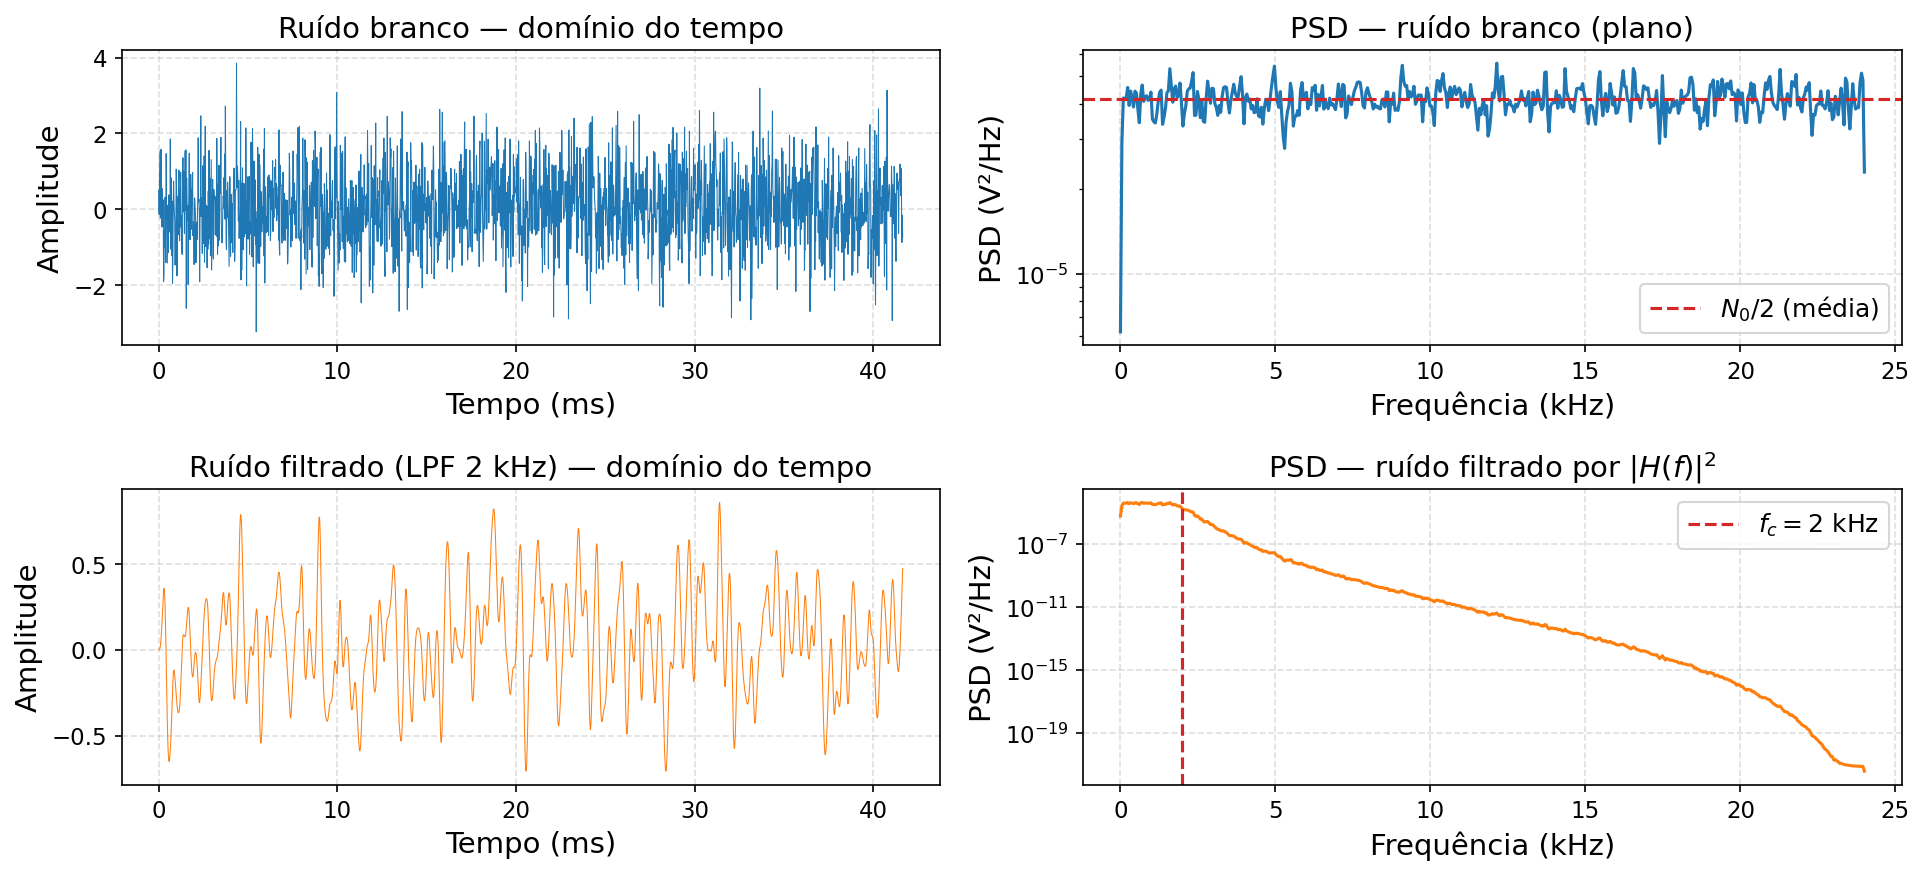
\includegraphics[width=\figFull, height=0.85\textheight, keepaspectratio]{figures/cap3/ruido_branco_filtrado}
\end{center}

\end{frame}

% ============================================

\begin{frame}{Exemplo: Ruído em Filtro RC}

\textbf{Filtro:} $H(\omega) = 1/(1 + j\omega RC)$, \quad $\omega_c = 1/(RC)$

\textbf{Entrada:} Ruído branco $S_n = N_0/2$

\textbf{PSD na saída:}
\[
S_y(\omega) = \frac{N_0/2}{1 + (\omega RC)^2}
\]

\textbf{Potência na saída:}
\[
P_y = \frac{1}{2\pi} \int_{-\infty}^{\infty} \frac{N_0/2}{1 + (\omega/\omega_c)^2}\, d\omega = \frac{N_0}{4\pi} \cdot \pi\omega_c = \frac{N_0\omega_c}{4} = \frac{N_0}{4RC}
\]

Potência de ruído na saída \textbf{proporcional à largura de banda} do filtro.

\end{frame}

% ============================================

\begin{frame}{Relação Sinal-Ruído (SNR)}

\[
\text{SNR} = \frac{P_{\text{sinal}}}{P_{\text{ruído}}}, \qquad \text{SNR}_{\text{dB}} = 10\log_{10}\!\left(\frac{P_s}{P_n}\right)
\]

\textbf{Sistema com filtro passa-baixas ideal de largura $B$ (Hz):}

\begin{itemize}
\item Potência do sinal: $P_s$ (assumindo sinal banda-limitada)
\item Potência do ruído: $P_n = N_0 B$
\end{itemize}

\[
\text{SNR} = \frac{P_s}{N_0 B}
\]

\textbf{Compromisso:} Aumentar $B$ pode aumentar capacidade, mas aumenta ruído.

\end{frame}

% ============================================

\begin{frame}{Exemplo: Link de Comunicação Wi-Fi}

\textbf{Parâmetros típicos (802.11n):}

\begin{itemize}
\item Potência transmitida: $P_t = 20$ dBm (100 mW)
\item Banda: $B = 20$ MHz
\item Ruído térmico: $N_0 = kT = 4 \times 10^{-21}$ W/Hz
\end{itemize}

\textbf{Potência de ruído na banda:}
\[
P_n = N_0 B = 4 \times 10^{-21} \times 20 \times 10^6 = 8 \times 10^{-14} \text{ W} = -101 \text{ dBm}
\]

\textbf{Se atenuação do canal é 60 dB} (distância $\sim$10 m):

$P_r = 20 - 60 = -40$ dBm

$\text{SNR} = -40 - (-101) = 61$ dB $\Rightarrow$ excelente qualidade!

\end{frame}

% ============================================

\begin{frame}{Resumo: Energia, Potência e Densidades Espectrais}

\begin{center}
\renewcommand{\arraystretch}{1.4}
\begin{tabular}{|l|c|c|}
\hline
& \textbf{Sinal de Energia} & \textbf{Sinal de Potência} \\ \hline
\textbf{Grandeza} & $E = \int |f(t)|^2 dt$ & $P = \lim \frac{1}{T}\int |f(t)|^2 dt$ \\ \hline
\textbf{Dens. Espectral} & $\Psi(\omega) = |F(\omega)|^2$ & $S(\omega) = \lim \frac{|F_T(\omega)|^2}{T}$ \\ \hline
\textbf{Autocorrelação} & $R(\tau) = \int f(t) f^*(t-\tau) dt$ & $R(\tau) = \lim \frac{1}{T}\int f f^* dt$ \\ \hline
\textbf{Wiener-Khinchin} & $R(\tau) \leftrightarrow \Psi(\omega)$ & $R(\tau) \leftrightarrow S(\omega)$ \\ \hline
\textbf{Saída canal} & $\Psi_y = |H|^2 \Psi_x$ & $S_y = |H|^2 S_x$ \\ \hline
\end{tabular}
\end{center}

\vspace{0.2cm}

\textbf{Resultados-chave:}

\begin{itemize}
\item Canal multiplica a densidade espectral por $|H(\omega)|^2$
\item Ruído de saída: $P_n = N_0 B$ (proporcional à banda)
\item Relação de incerteza: $\Delta t \cdot \Delta \omega \geq 1/2$
\end{itemize}

\end{frame}
